\documentclass{standalone}
\usepackage{tikz}
\usepackage{graphicx}

\begin{document}
  \begin{tikzpicture}
    % Load PDF image
    \node[anchor=south west,inner sep=0] (image) at (0,0) {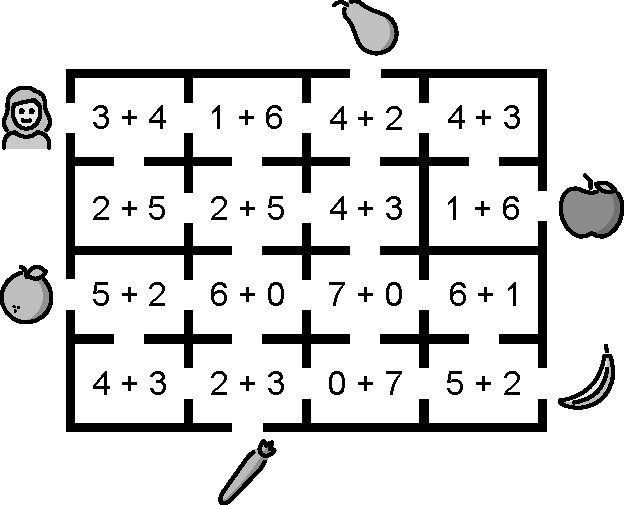
\includegraphics[width=\textwidth]{P12gs.pdf}};
    
    % Draw arrow
    \draw[ultra thick, ->] (1.1,7.5) -- (1.6,7.5);
    
    \node[fill=white, opacity=1, text opacity=1, inner sep=1pt] at (2.5,7.5) {{\huge $3+4$}};
    \node[fill=white, opacity=1, text opacity=1, inner sep=1pt] at (4.75,7.5) {{\huge $1+6$}};
    \node[fill=white, opacity=1, text opacity=1, inner sep=1pt] at (7.1,7.5) {{\huge $4+2$}};
    \node[fill=white, opacity=1, text opacity=1, inner sep=1pt] at (9.4,7.5) {{\huge $4+3$}};
    \node[fill=white, opacity=1, text opacity=1, inner sep=1pt] at (2.5,5.8) {{\huge $2+5$}};
    \node[fill=white, opacity=1, text opacity=1, inner sep=1pt] at (4.75,5.8) {{\huge $2+5$}};
    \node[fill=white, opacity=1, text opacity=1, inner sep=1pt] at (7.1,5.8) {{\huge $4+3$}};
    \node[fill=white, opacity=1, text opacity=1, inner sep=1pt] at (9.4,5.8) {{\huge $1+6$}};
    \node[fill=white, opacity=1, text opacity=1, inner sep=1pt] at (2.5,4.1) {{\huge $5+2$}};
    \node[fill=white, opacity=1, text opacity=1, inner sep=1pt] at (4.75,4.1) {{\huge $6+0$}};
    \node[fill=white, opacity=1, text opacity=1, inner sep=1pt] at (7.1,4.1) {{\huge $7+0$}};
    \node[fill=white, opacity=1, text opacity=1, inner sep=1pt] at (9.4,4.1) {{\huge $6+1$}};
    \node[fill=white, opacity=1, text opacity=1, inner sep=1pt] at (2.5,2.4) {{\huge $4+3$}};
    \node[fill=white, opacity=1, text opacity=1, inner sep=1pt] at (4.75,2.4) {{\huge $2+3$}};
    \node[fill=white, opacity=1, text opacity=1, inner sep=1pt] at (7.1,2.4) {{\huge $0+7$}};
    \node[fill=white, opacity=1, text opacity=1, inner sep=1pt] at (9.4,2.4) {{\huge $5+2$}};
  \end{tikzpicture}
\end{document}